\section{Experimental Results}
\label{sec:exp}

In this section, we conduct experiments on a synthetic data set and a real data set 
to verify the effectiveness of our proposed worker model and debiasing technique.  

\subsection{Data sets}
We first introduce the data sets we used in this experiments.  
A summary of the data sets we used in our experiments are given in Table~\ref{tab:dataset}.  

\vpara{Synthetic.}
We construct synthetic data sets following the worker annotation model we proposed in Section~\ref{sec:worker}.
Suppose we have $n$ items in $X$, 
we first generate their predictive probability $\eta_i$ for each $x_i \in X$ 
from a Beta distribution $Beta(\alpha, \beta)$, 
then generate the true labels $Y$ by drawing $y_i$ from a Bernoulli distribution parameterized by $\eta_i$ for each $i$.  
In our synthetic data set, we set $\alpha = 2$ and $\beta = 4$ to simulate the case when negative data items overwhelm.

Then we generate $m$ batches of size $k$ by sampling without replacement for each batch.  
Notice that by ``without replacement'' we mean there are no identical data items within the same batch, 
while the same item can still appear in multiple batches 
as we do replace the items back into the pool after a batch is generated.  
Thereby we obtain the set of batches $B$.  
For each $b_j$ in $B$, we generate the workers' annotation $y_j'$ from our proposed batch annotation model.  
The probability of making independent judgments $\lambda$ is given.
The distribution of determining number of positive annotations $p_{\tau}$ is also assigned to be:
\beal{
	p_{\tau} \propto (\tau + 1)^{- \rho} \nonumber
}%
where $\rho$ is positive constant.  
In our synthetic data set, we set $\lambda = 0.5$ and $\rho = 2$.  

\vpara{Comments.}
We utilize a real world crowdsourcing data set.  
The original crowdsourced task is to identify inappropriate comments on LinkedIn posts published by companies or LinkedIn influencers.  
Inappropriate comments are defined as comments containing promotional, profane, blatant soliciting, random greeting comments, 
as well as comments with \emph{only} web links and contact information.  
In order to collect annotation of comments, 
for each post, $k$ comments are sampled and sent to CrowdFlower as a batch (unit).  
Workers are also provided with a codebook (instruction) explaining how to annotate the data.  
Each comment is regarded as a data item and can be annotated as positive (inappropriate comment) or negative (acceptable comment).  
Each batch is annotated by more than 5 workers.  

In order to provide test questions and track the performance of each worker, 
some of the batches are annotated by 9 trained LinkedIn employees (experts) with the same codebook and interface as used for crowd workers.  
The average Cohen's kappa for all expert pairs is 0.7881.  
For this experiments, we only adopt the batches with all of their data items annotated by both crowds and experts 
as we can use the experts' annotation as ground truth (aggregated by majority voting).  
Among which, 1,099 batches that are annotated before a worker actually works on the job 
are utilized as training data set $B_L$.  
while the other 5,267 batches are utilized as test data set $B_U$ to infer the 651 data items they covered.  


\begin{table}[!t]
\centering
 {\caption{Data set statistics.}\label{tab:dataset}}
{
  \begin{tabular}{c||c|c|c|c|c}
  \hline
  Data set & $k$ & $n_L$  &  $m_L$ & $n_U$  & $m_U$ \\ \hline \hline
 Synthetic & 5 & 1,000 & 10,000 & 5,000 & 50,000 \\ \hline 
 Comments  & 5 & 110   & 1,099  & 651   & 5,267  \\ \hline  
  \end{tabular}
}
\end{table}


\subsection{Experimental Setup}

\vpara{Comparing method.}
We compare the performance of our proposed method with several baselines:
\begin{itemize}
  \item \emph{Majority Voting (MV)}.
        For each data item in the test data set, 
        simply determine its inferred label by the way it is annotated by the majority of workers.  
        This aggregation strategy is adopted by many crowdsourcing service.  
  \item \emph{Majority Voting with Tuned Threshold (MVT)}.
        Instead of simply applying majority voting, 
        we calculate the ratio of positive annotation on each item as a score, 
        and tune the threshold for determining the binary inferred label.  
        Based on a given training set of annotation and true labels, 
        we find the threshold yielding the best $F_1$-score on training data set, 
        and apply the same threshold on the test data set.  
  \item \emph{Plackett-Luce Model (PL)}.  
        A strategy is to fit the Plackett-Luce model on the test data by inferring the scores $s(x_i)$ associated with each data items.  
        We apply a Bayesian regularization on the inferred scores to confine it as $0 \leq s(x_i) \leq 1$.  
        We then infer a positive label to each data item with an inferred score $s(x_i) > 0.5$ and a negative label otherwise.  
  \item[*] \emph{Batch Annotation Model (BAM)}.  
        The debiasing strategy proposed in Section~\ref{sec:worker} and~\ref{sec:debias}.
\end{itemize}

\vpara{Evaluation.}
For baselines without training, we directly apply them on the test data set; 
for our proposed method, we first train the worker model on the training data set, 
then apply the debiasing strategy based on the trained worker model on the test data set.  
We compare the inferred labels to the ground-truth and evaluate the performance in terms of accuracy, precision, recall and $F_1$-score.  
As all the methods generate scores for each data item 
(for MV we take the proportion of workers who annotated a data item as positive as the inferred score),
we also evaluate the performance in terms of the area of ROC curves.  


\vpara{Experimental setup.}
For our proposed model, 
in training phase, we initialize $\lambda$ to be 0.5 and $p_{\tau}$ to be a random value between 0 and 1;
in debiasing phase, we initialize the all the inferred scores as $0.1$. 
For training the worker model, we set a fixed number of iteration as 100.  
Our experimental results presented later show the model converge within number of iterations much fewer than 100.  
For debiasing, we calculate the log-likelihood of the model and stop when the relative change of log-likelihood is within 0.001.  


\subsection{Experimental Results}


\vpara{Worker model learning.}
We first verify the effectiveness of learning our proposed worker model.  
On synthetic data set, the ``true'' value of probability of making independent judgments $\lambda$ is set to 0.5.  
We learn the model from the synthetic training data and obtain the inferred $\hat{\lambda}$ as 0.4998, 
which reasonably recovers the original value.  
We also compare the original model parameters $p_{\tau}$'s to the inferred parameters in Figure~\ref{subfig:p_tau_synthetic}.  
The black dash line represents the original parameters used for generating synthetic annotation data, 
while the red solid line shows the inferred parameters of worker model, 
which seems as a precise fit of the original parameter.  
We also show the curve of log-likelihood of the training data set,
which seems to converge within 20 iterations.  

To further confirm the robustness of our learning method, 
we modify the configuration of synthetic data generation, 
and train the worker model on different data sets to check if they can recover the original parameters.  
We still take the same configuration of $n_L = 1,000$ and $m_L = 10,000$.  
The estimation error analysis is shown in Figure~\ref{fig:esterr}.  
Figure~\ref{subfig:lambda_esterr} shows the difference between the inferred parameter $\hat{\lambda}$ 
and the ``true'' parameter $\lambda$, 
given the annotation data generated by $\lambda$ varying from 0.1 to 0.9.  
It can be observed that the error is reasonable small, basically within 0.1.  
Figure~\ref{subfig:ptau_esterr} shows the $\ell_2$ norm of the difference between the estimated distribution $\hat{p}_{\tau}$
and the ``true'' distribution $p_{\tau}$, 
when $p_{\tau}$ is generated with respect to different $\rho$ varying from 1 to 3.  
In most of the settings, the error is below $2 \times 10^{-3}$.  
The error is basically tolerable.  
Although we only instantiate $p_{\tau}$'s by power-law distribution, 
as the learning method does not confine the learned distribution to be parametric, 
it can be directly applied to any other type of distributions.  



\begin{figure}[!t]
  \centering
  \subfigure[Parameter comparison of $p_{\tau}$'s]{
    \label{subfig:p_tau_synthetic}
    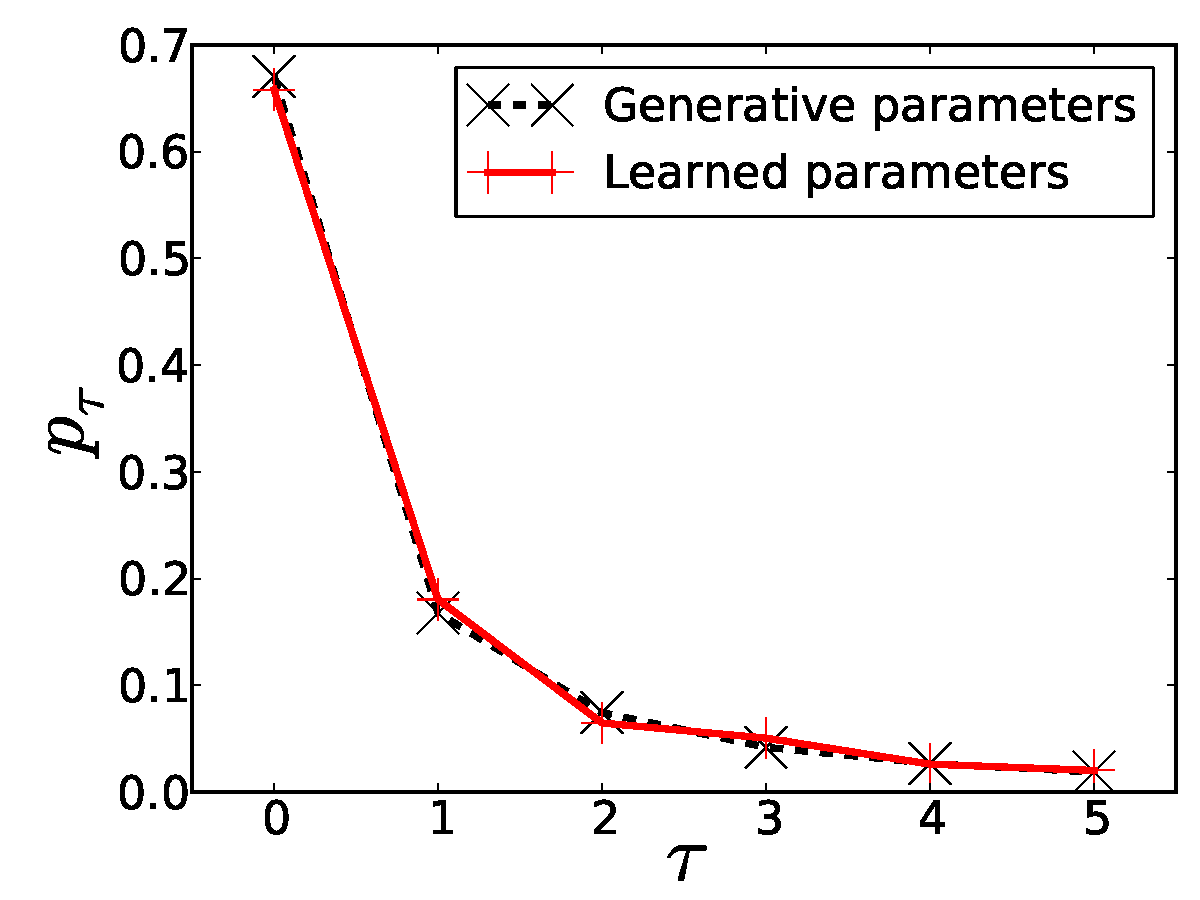
\includegraphics[width=0.46\columnwidth]{figures/ptau_synthetic}
  }
  \subfigure[Convergence analysis]{
    \label{subfig:convergence_synthetic}
    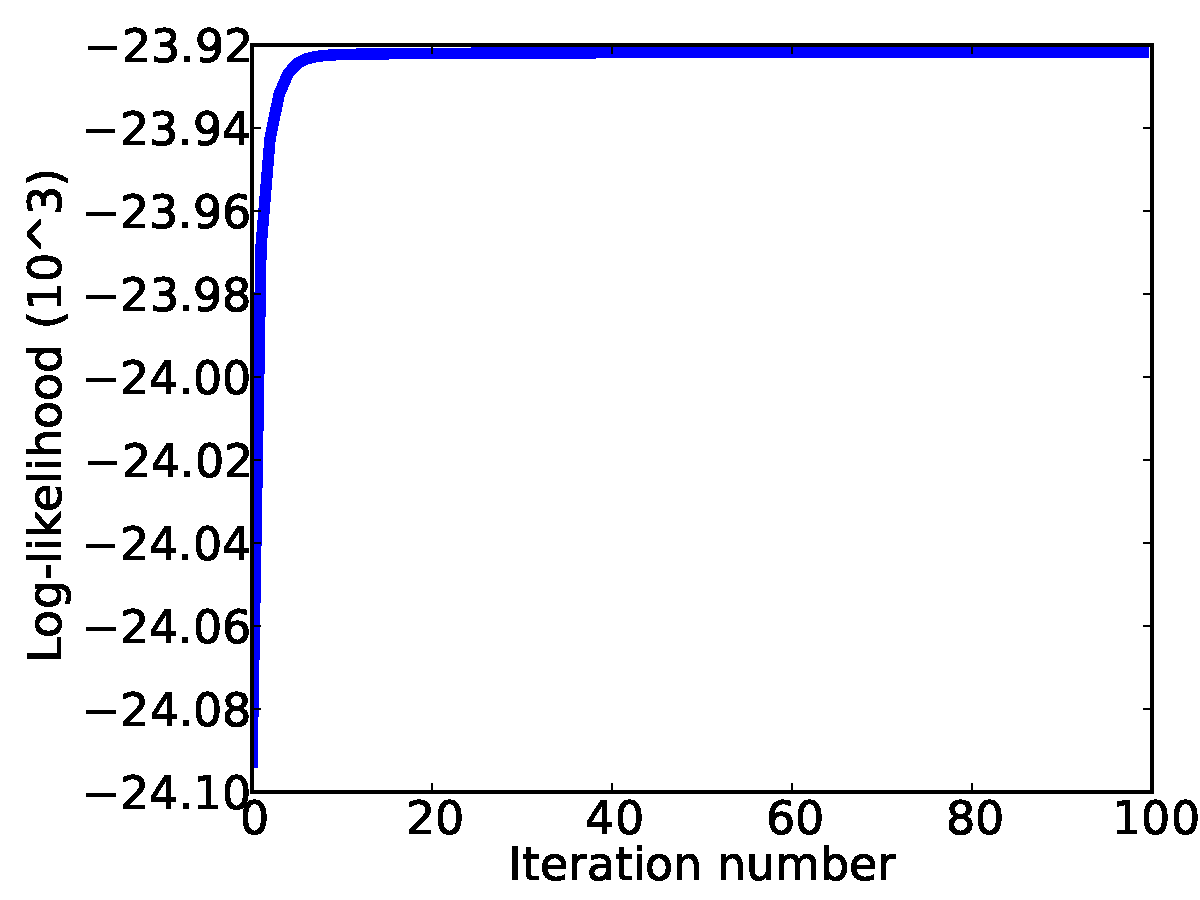
\includegraphics[width=0.46\columnwidth]{figures/loglikelihood_synthetic}
  }
  \caption{\label{fig:synthetic_training}
  Learning worker model from the synthetic training data set.
  }
\end{figure}

\begin{figure}[!t]
  \centering
  \subfigure[Estimation error of $\lambda$]{
    \label{subfig:lambda_esterr}
    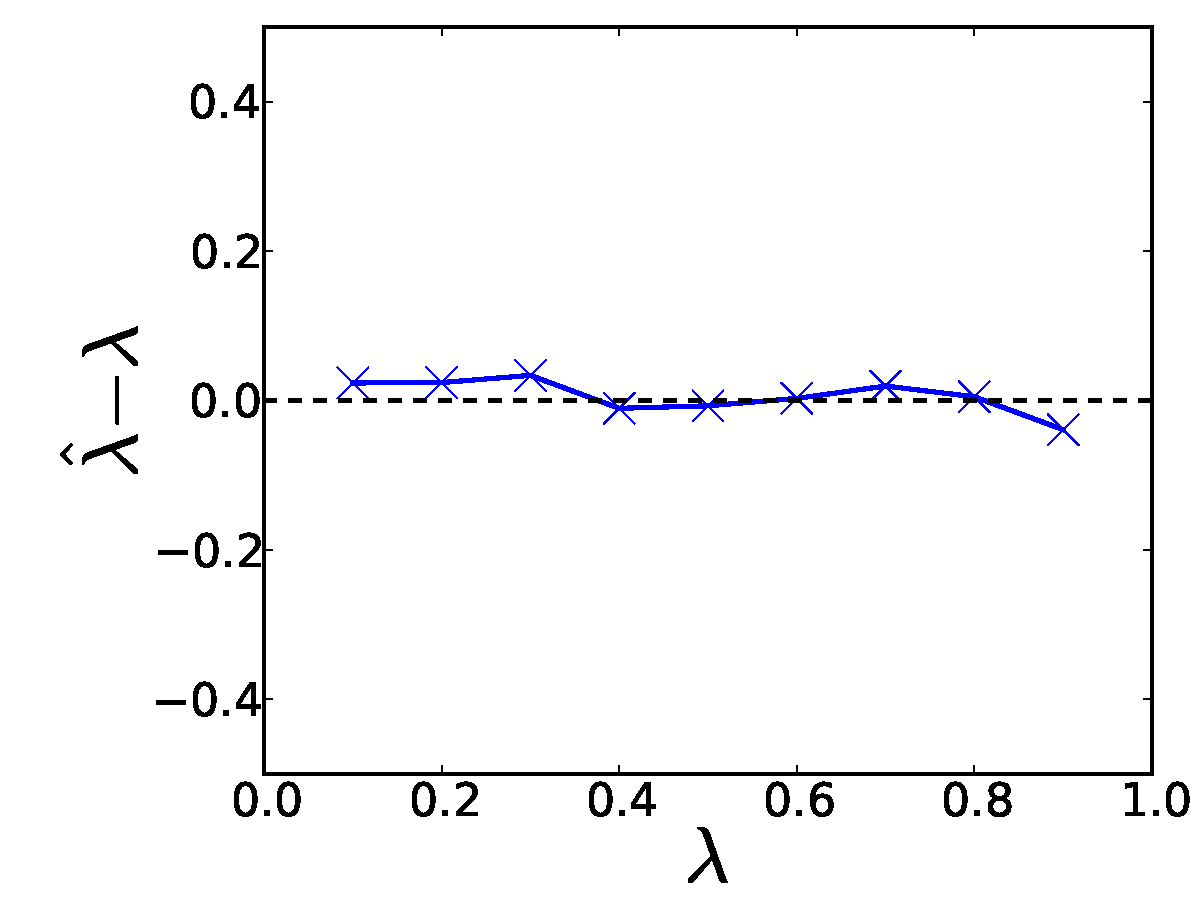
\includegraphics[width=0.46\columnwidth]{figures/lambda_esterr}
  }
  \subfigure[Estimation error of $p_{\tau}$]{
    \label{subfig:ptau_esterr}
    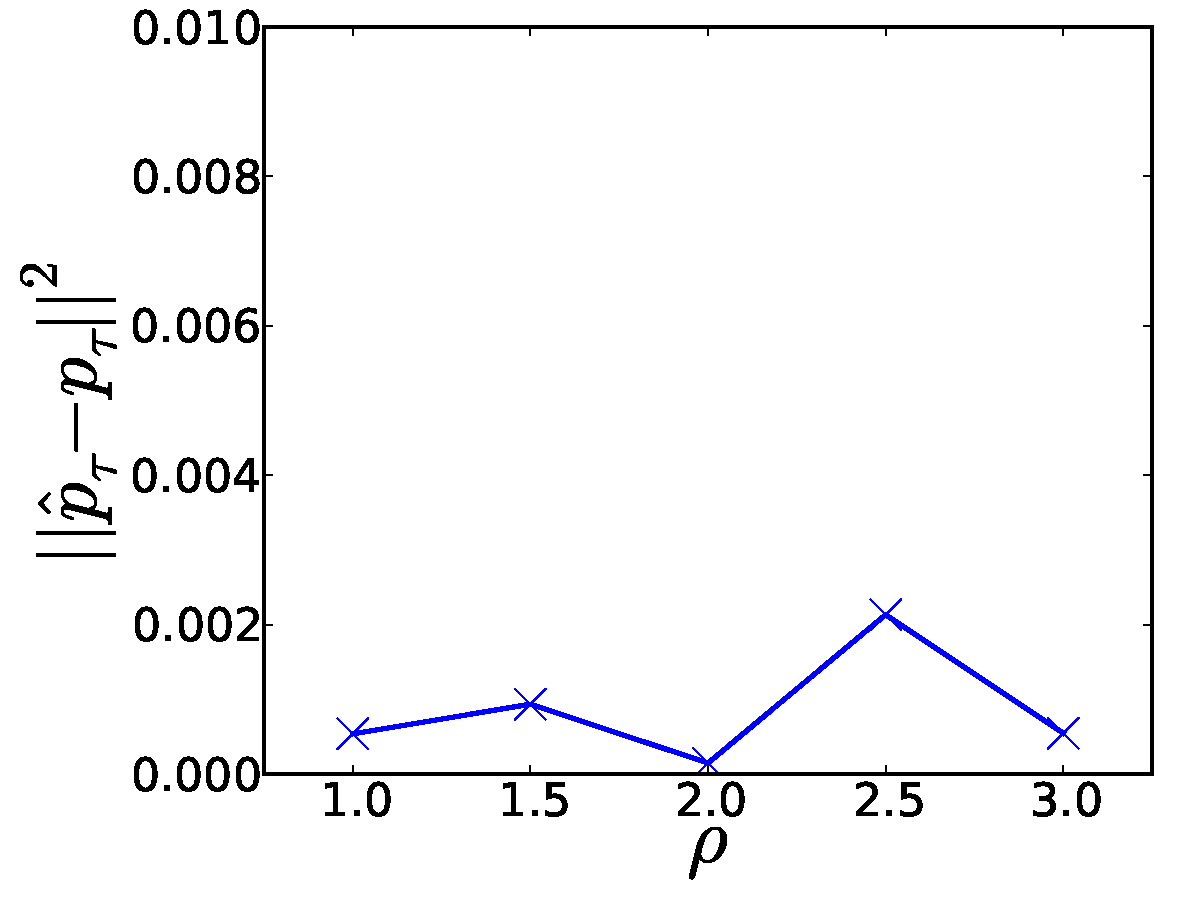
\includegraphics[width=0.46\columnwidth]{figures/ptau_esterr}
  }
  \caption{\label{fig:esterr}
  Analysis of estimation error of parameters in the worker model under different configurations. 
  }
\end{figure}



\vpara{Learned model on real data set.}
Given the effectiveness of our learning method verified, 
we apply the worker model trying to fit the data set of annotating inappropriate comments.  
The learned probability of a worker making independent judgments $\hat{\lambda}$ is 0.7877.  
The learned distribution for determining the number of positive annotation in a batch is presented in Figure~\ref{subfig:p_tau_lnkd}.  
It shows that a worker tends to annotate the entire batch as negative (\ie~acceptable comment) with a probability over 0.6, 
while picking only 1 of them as positive (\ie~inappropriate comment) also occurs with a relative high probability around 0.25.  
The workers seem to be reluctant to annotate more than 1 comments in a size-5 batch.  
This is coherent with most people's intuition that inappropriate comments are rare comparing to the entire set of comments.  

The convergence analysis is shown in Figure~\ref{subfig:convergence_lnkd}.  
The model converges within 50 iterations.  


\begin{figure}[!t]
  \centering
  \subfigure[Parameter analysis of $p_{\tau}$'s]{
    \label{subfig:p_tau_lnkd}
    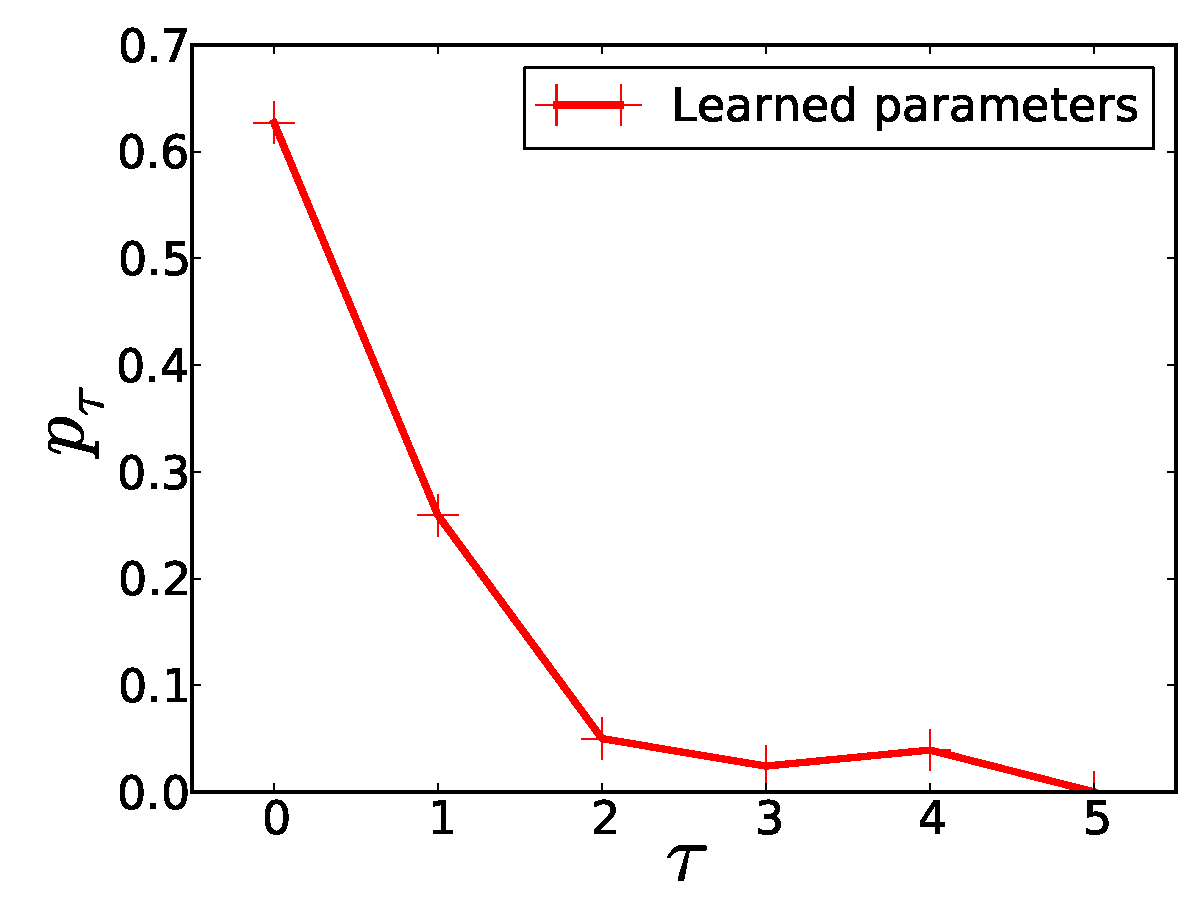
\includegraphics[width=0.46\columnwidth]{figures/ptau_lnkd}
  }
  \subfigure[Convergence analysis]{
    \label{subfig:convergence_lnkd}
    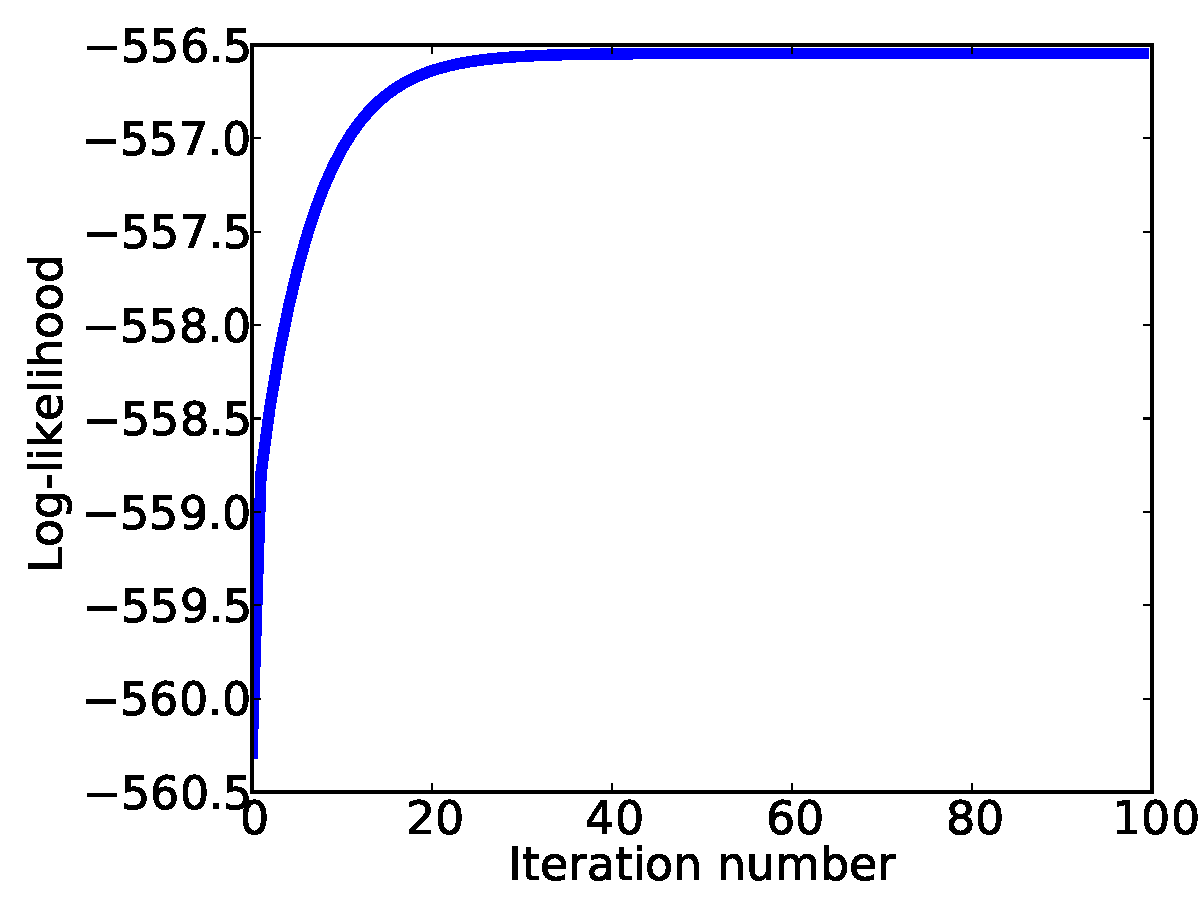
\includegraphics[width=0.46\columnwidth]{figures/loglikelihood_lnkd}
  }
  \caption{\label{fig:lnkd_training}
  Learning worker model from the comments training data set.
  }
\end{figure}


\vpara{Performance comparison.}
We proceed to evaluate the performance of different aggregation strategies on both data sets.  
The overall performance results are shown in Table~\ref{tab:performance}.  
In both data sets, our proposed debiasing strategy is a clear winner in terms of $F_1$-score, 
and also achieves the best accuracies.  

In synthetic data set, majority voting, without tuning the threshold (default set to 0.5), fails to identify most of the positive data items, 
and therefore achieves an extremely low recall.  
Only after the threshold is tuned on a training data set 
can it achieve a reasonable $F_1$-score of 71\%.  
%Although in practices one can usually achieve a better performance by adjusting the threshold of assigning a positive label, 
%the determination of the threshold is usually empirical without a clear guideline.  
PL-model, in contrast, achieves a relatively low precision of 52\%.  
Our proposed method is proven to achieve the best overall performance in terms of $F_1$-score and accuracy, 
and the precision and recall achieved by our method are also relatively balanced.  
Notice that we do not directly apply any threshold tuning for our method and simply takes the threshold as 0.5.  

In comments data set, na\"{i}ve majority voting strategy again obtains a poor recall below 80\%, 
After tuning the threshold, its recall rises to around 85\%, but still lower than our proposed method.  
The scores learned by PL-model yield a comparable recall to majority voting with tuned threshold, 
but fail to achieve a high precision.  
Our proposed method achieves a comparable precision of 93\% and a higher recall of 87\%, 
and therefore beat all the other baselines in terms of $F_1$-score (90\%).  


It is worth noting that in both data sets, the AUC of all the methods are comparable.  
This implies the quality of ranking recovered by all the methods are similar.  
However, to obtain reliable annotations, it is non-trivial and critical problem to accurately infer the scales of scores 
or to pick a reasonable threshold.  

% The strategy of determining the threshold for differentiating positive and negative data items makes the difference.  


\begin{table}[!t]
\centering
 {\caption{Performance comparison of Majority Voting (MV), Plackett-Luce Model (PL) and Batch Annotation Model (BAM).  
 All results are shown as percents.}\label{tab:performance}}
{

  \begin{tabular}{@{}c@{}|@{}c@{}||c|c|c|c|c@{}}
    \hline
        Data set & Method    & Acc.           & Prc.           & Rcl.           & $F_1$          & AUC \\ \hline \hline
        \multirow{4}{*}{Synthetic}
                 & MV        & 83.04          & \textbf{98.91} & 00.10          & 17.67          & 93.84          \\ \cline{2-7}
                 & MVT       & 88.06          & 64.69          & 80.06          & 71.56          & 93.84          \\ \cline{2-7}
                 & PL        & 82.74          & 52.25          & \textbf{92.75} & 66.85          & 94.46          \\ \cline{2-7}
                 & BAM       & \textbf{89.88} & 70.93          & 78.04          & \textbf{74.31} & \textbf{94.95} \\ \hline
        \multirow{4}{*}{Comments}
                 & MV        & 95.55          & \textbf{93.75} & 79.65          & 86.12          & 99.05          \\ \cline{2-7}
                 & MVT       & 96.16          & 92.31          & 84.96          & 88.48          & 99.05          \\ \cline{2-7}
                 & PL        & 94.62          & 85.45          & 83.19          & 84.30          & 96.40          \\ \cline{2-7}
                 & BAM       & \textbf{96.77} & 93.40          & \textbf{87.61} & \textbf{90.41} & \textbf{99.06} \\ \hline
  \end{tabular}
}
\end{table}
